\documentclass[14pt]{extreport}
\usepackage{cmap}
\usepackage[utf8]{inputenc}
\usepackage[english,ukrainian]{babel}
\usepackage{graphicx}
\usepackage{geometry}
\usepackage{listings}
\usepackage{amsmath}
\usepackage{float}
\usepackage{array}
\geometry{
	a4paper,
	left=20mm,
	right=20mm,
	top=20mm,
	bottom=20mm
}
\lstset{
	language=bash,
	tabsize=4,
	breaklines,
	keepspaces,
	showstringspaces=false,
}
\graphicspath{ {./pictures} }
\setlength{\parindent}{4em}

\newcommand\subject{Аналіз вимог до програмного забезпечення}
\newcommand\lecturer{професор кафедри ПЗ\\Грицюк Ю.І.}
\newcommand\teacher{асистент кафедри ПЗ\\Масюкевич В.В.}
\newcommand\mygroup{ПЗ-32}
\newcommand\lab{1}
\newcommand\theme{Аналіз наявних програм-аналогів для встановлення вимог до нового програмного забезпечення для обраної предметної області}
\newcommand\purpose{Проаналізувати наявні програмні продукти заданої предметної
	області}

\begin{document}
\begin{normalsize}
	\begin{titlepage}
		\thispagestyle{empty}
		\begin{center}
			\textbf{МІНІСТЕРСТВО ОСВІТИ І НАУКИ УКРАЇНИ\\
				НАЦІОНАЛЬНИЙ УНІВЕРСИТЕТ "ЛЬВІВСЬКА ПОЛІТЕХНІКА"}
		\end{center}
		\begin{flushright}
			Інститут \textbf{КНІТ}\\
			Кафедра \textbf{ПЗ}
		\end{flushright}
		\vspace{200pt}
		\begin{center}
			\textbf{ЗВІТ}\\
			\vspace{10pt}
			До лабораторної роботи № \lab\\
			\textbf{На тему}: “\textit{\theme}”\\
			\textbf{З дисципліни}: “\subject”
		\end{center}
		\vspace{40pt}
		\begin{flushright}
			
			\textbf{Лектор}:\\
			\lecturer\\
			\vspace{10pt}
			\textbf{Виконав}:\\
			
			студент групи \mygroup\\
			Коваленко Д.М.\\
			\vspace{10pt}
			\textbf{Прийняв}:\\
			
			\teacher\\
			
			\vspace{28pt}
			«\rule{1cm}{0.15mm}» \rule{1.5cm}{0.15mm} 2023 р.\\
			$\sum$ = \rule{1cm}{0.15mm}……………\\
			
		\end{flushright}
		\vspace{\fill}
		\begin{center}
			\textbf{Львів — 2023}
		\end{center}
	\end{titlepage}
		
	\begin{description}
		\item[Тема.] \theme.
		\item[Мета.] \purpose.
	\end{description}

	\section*{Лабораторне завдання}
	\begin{enumerate}
		\item Вибрати предметну область із запропонованого переліку.
		\item Здійснити пошук в мережі Інтернет кількох (від трьох до п'яти) наявних
		програм-аналогів для обраної предметної області. Якщо у вільному доступі немає
		програм-аналогів, проаналізувати вітчизняні та закордонні веб-ресурси.
		\item Описати кожну із розглянутих програмних систем (сайтів).
		\item Здійснити порівняння наявних програм-аналогів і внести дані в таблицю.
		\item На основі проведеного аналізу скласти перелік вимог до ПС для заданої
		предметної області.
		\item Оформити звіт.
	\end{enumerate}
	
	\section*{Хід роботи}
	
	\subsection*{EcoLane}
	\textit{EcoLane} - це програмна система для управління транспортними послугами, яка допомагає організовувати та відстежувати маршрути та розклади громадського транспорту, оптимізувати маршрутизацію, інтегрувати електронні квитки та покращувати доступність громадського транспорту для пасажирів.
	
	\begin{figure}[H]
		\centering
		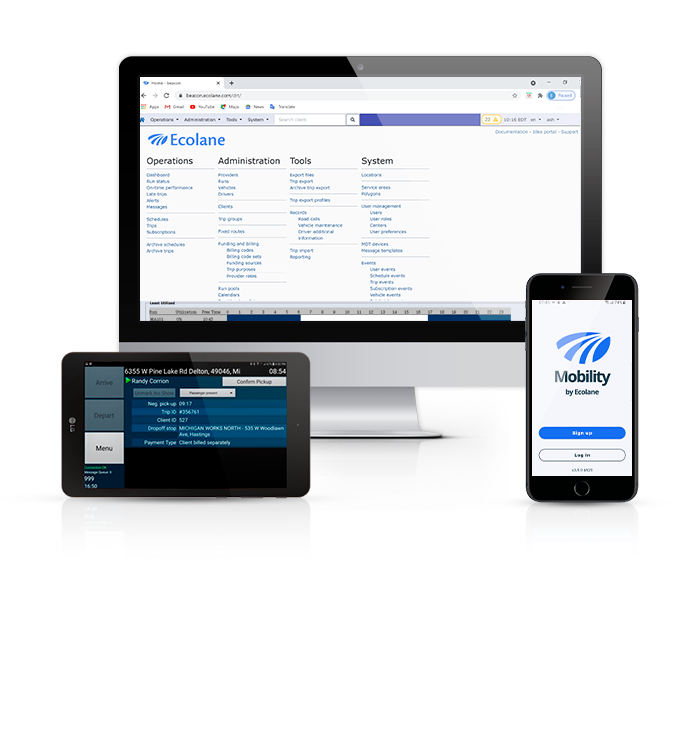
\includegraphics[trim={0 8cm 0 2cm},clip,scale=0.7]{1}
		\caption{EcoLane}
	\end{figure}
	
	\textbf{Основні функціональні можливості та переваги}:
	\begin{itemize}
		\item Окремий додаток для пасажирів з можливістю бронювання місць та оплати проїзду.
		\item Можливість автоматизованої побудови оптимального маршруту.
		\item Формування даних для аналітики ефективності.
		\item Безкоштовна цілодобова технічна підтримка.
		\item Можливість відслідковувати рух транспорту
		\item Інтеграція з Google Maps для отримання розкладу руху та відстеження транспорту.
		\item Простий веб-інтерфейс, що не вимагає встановлення будь-якого програмного забезпечення.
		\item Можливість автоматичної генерації оптимального розкладу руху транспорту.
	\end{itemize}
	
	\subsection*{TransLoc}
	\textit{TransLoc} - це система громадського транспорту, яка забезпечує розклад руху автобусів та інших транспортних засобів, а також надає інформацію про їхнє місцезнаходження в режимі реального часу. Вона дозволяє пасажирам відстежувати рух транспорту через мобільний додаток або інтернет, щоб зручно та ефективно планувати свої поїздки.
	
	\begin{figure}[H]
		\centering
		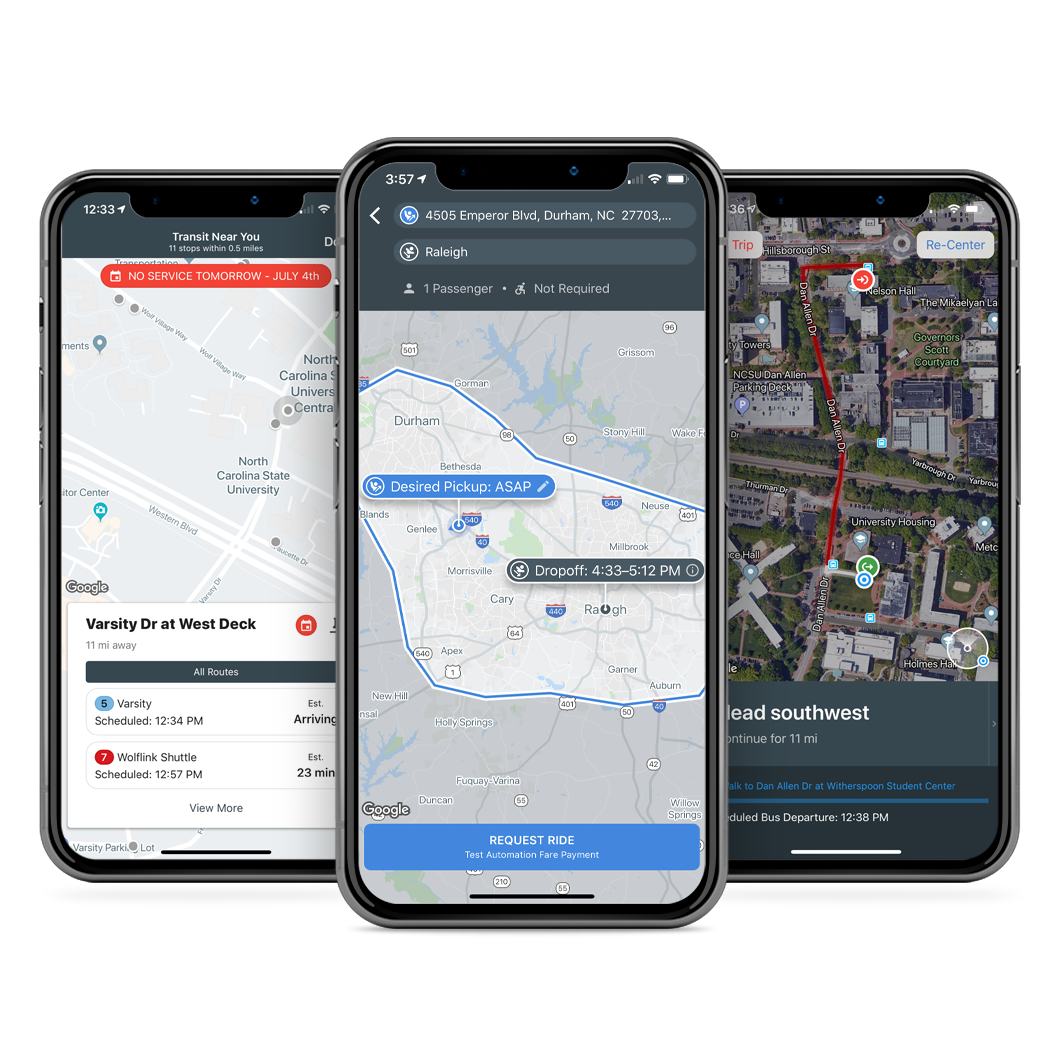
\includegraphics[scale=0.45]{4}
		\caption{TransLoc}
	\end{figure}
	
	\textbf{Основні функціональні можливості та переваги}:
	\begin{itemize}
		\item Окремий додаток для водія.
		\item Можливість комунікувати з водієм за допомогою додатку.
		\item Можливість автоматизованої побудови оптимального маршруту.
		\item Можливість відслідковувати рух транспорту.
		\item Простий веб-інтерфейс, що не вимагає встановлення будь-якого програмного забезпечення.
	\end{itemize}
	
	\textbf{Недоліки}:
	\begin{itemize}
		\item Відсутність можливості генерації розкладу руху транспорту.
	\end{itemize}
	
	\subsection*{OptiBus}
	\textit{OptiBus} - це сучасна інтегрована система для управління громадським транспортом, яка дозволяє оптимізувати маршрути, розклади, ресурси та забезпечує ефективне управління транспортними операціями, сприяючи покращенню якості та доступності громадського транспорту.
	
	
	\begin{figure}[H]
		\centering
		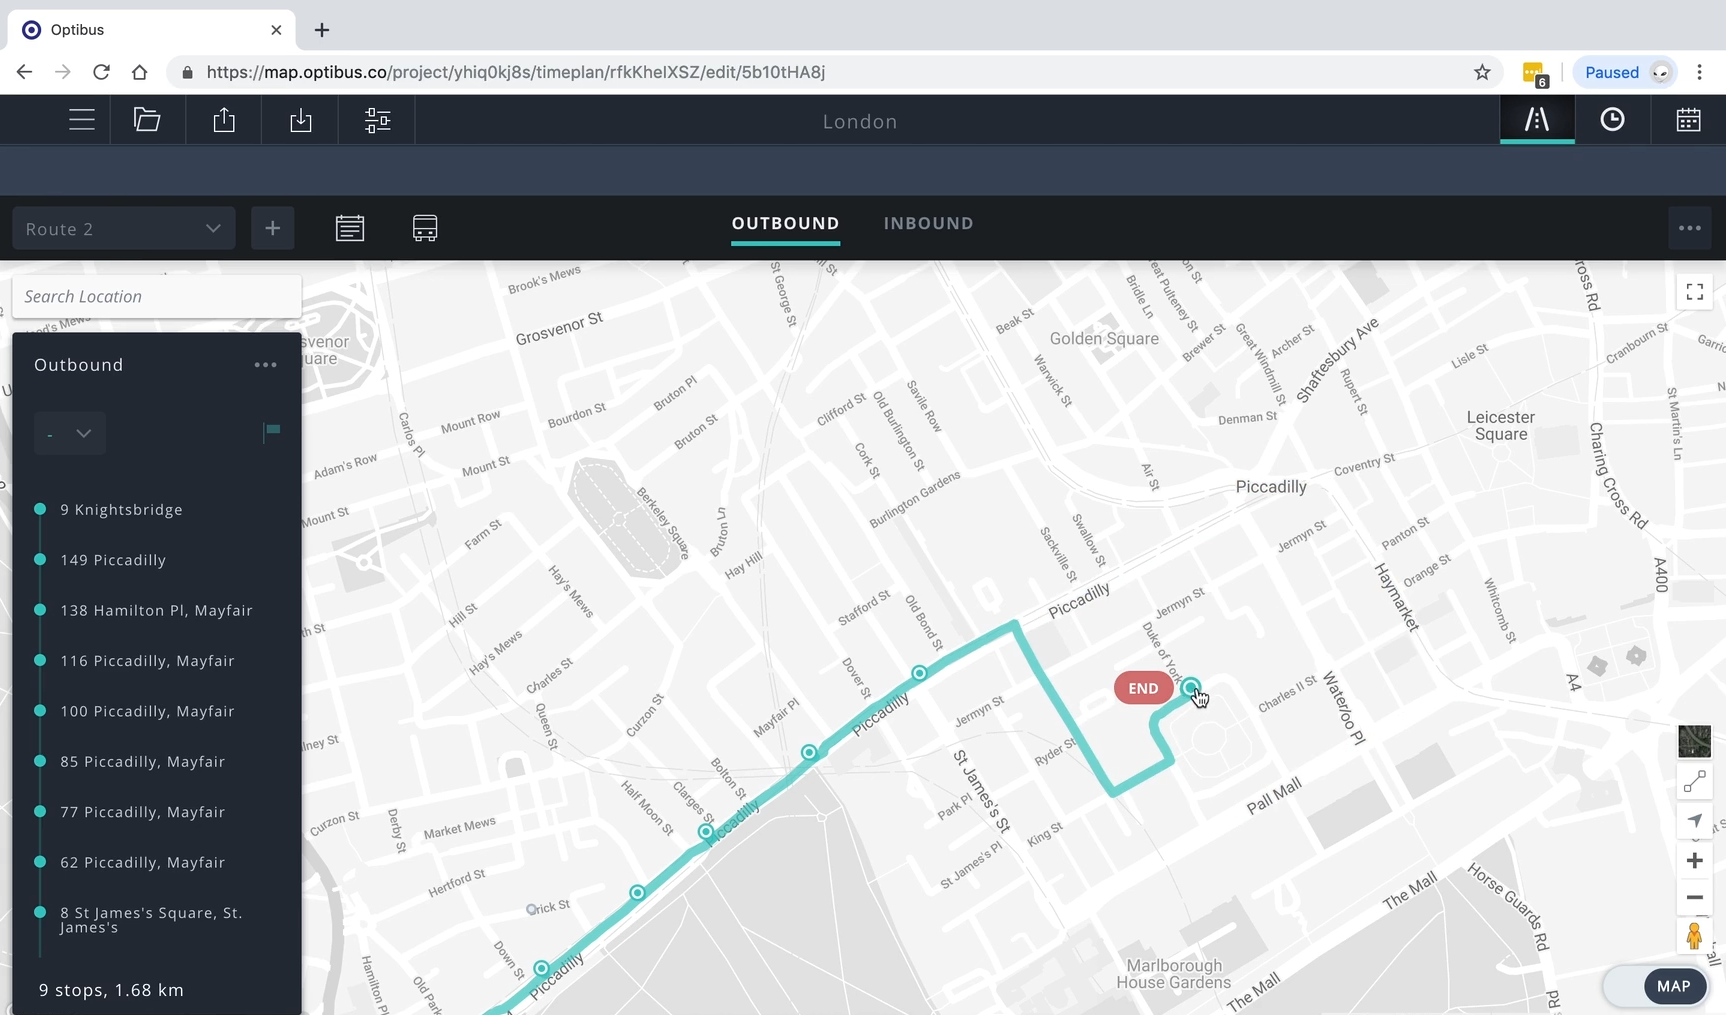
\includegraphics[scale=0.25]{3}
		\caption{OptiBus}
	\end{figure}
	
	\textbf{Основні функціональні можливості та переваги}:
	\begin{itemize}
		\item Формування даних для аналітики ефективності.
		\item Окремий додаток для пасажирів з можливістю бронювання місць.
		\item Можливість комунікації з пасажирами за допомогою додатку.
		\item Простий єдиний веб-інтерфейс для пасажирів, водіїв та компанії, що не вимагає встановлення будь-якого програмного забезпечення.
		\item Можливість автоматизованої побудови оптимального маршруту.
		\item Можливість автоматичної генерації оптимального розкладу руху транспорту.
	\end{itemize}
	
	\subsection*{Беспалов ЛАБ}
	\textit{Беспалов ЛАБ} - платформа для створення транспортних моделей міст, країн і цілих регіонів. Інструмент оптимізації й оцінки прибутковості громадського транспорту.
	
	\begin{figure}[H]
		\centering
		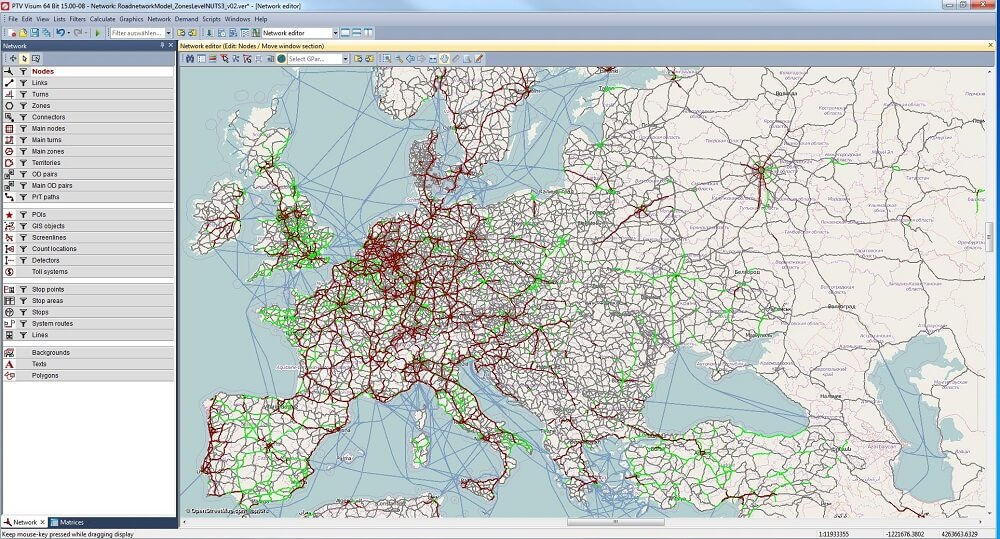
\includegraphics[scale=0.45]{2}
		\caption{Беспалов ЛАБ}
	\end{figure}
	
	\textbf{Основні функціональні можливості та переваги}:
	\begin{itemize}
		\item Моделювання транспортних моделей для визначення найоптимальніших маршрутів.
		\item Формування даних для аналітики та оптимізації транспорту.
	\end{itemize}
	
	\textbf{Недоліки}:
	\begin{itemize}
		\item Відсутність можливості генерації розкладу руху.
		\item Відсутність можливості автоматичної побудови маршрутів.
	\end{itemize}
	
	\begin{table}[H]
		\centering
		\renewcommand*\arraystretch{1.3}
		\begin{tabular}{|p{0.26\linewidth}|p{0.13\linewidth}|p{0.14\linewidth}|p{0.13\linewidth}|p{0.22\linewidth}|}
			\hline
			 & \textbf{EcoLane} & \textbf{TransLoc} & \textbf{OptiBus} & \textbf{Беспалов ЛАБ}\\\hline
			\textbf{Інтерфейс} & Веб і вбудована система & Веб і моб. додаток & Веб & Win7+ \\\hline
			\textbf{Вимагає підключення до мережі} & Так & Так & Так & Ні\\\hline
			\textbf{Оновлення системи} & Так & Так & Так & Так\\\hline
			\textbf{Зв'язок з банківською системою для оплати} & Так & Ні & Ні & Ні\\\hline
			\textbf{Відслідковування транспорту за допомогою GPS} & Так & Так & Ні & Ні\\\hline
			\textbf{Вартість} & Індивіду-\newline альн & Індивіду-\newline альна & Індивіду-\newline альна & Індивіду-\newline альна\\\hline
			\textbf{Технічне обслуговування} & Так & Так & Ні & Так (обмежене в часі)\\\hline
			\textbf{Пробний режим роботи} & Онлайн демонстрація & Ні & Онлайн демонстрація & Ні\\\hline
		\end{tabular}
	\end{table}
	
	Порівнявши програмні системи, що є аналогами для системи управління компанії з регулярних перевезень, я можу виділити такі суттєві вимоги до цієї предметної області.
	\begin{itemize}
		\item Зручний інтерфес для використання адміністраторами системи, водіями та пасажирами.
		\item Інтеграція з банківською системою для оплати проїзду.
		\item Відслідковування транспорту за допомогою GPS.
		\item Інтеграція з Google Maps для отримання розкладу руху та відслідковування транспорту.
		\item Можливість бронювання квитків пасажирами.
		\item Можливість автоматизованої побудови оптимального маршруту.
		\item Можливість автоматичної генерації оптимального розкладу руху транспорту.
	\end{itemize}

	\section*{Висновок}
	Під час виконання лабораторної роботи я проаналізував програмні продукти, що є аналогами системи управління компанії з регулярних перевезень. Я виділив основний функціонал програмних продуктів, вивів їх переваги і недоліки. Також, порівняв продукти між собою та склав список головних вимог до цієї предметної області.
	 
\end{normalsize}
\end{document}
